% gap between figure 
\pgfplotsset{width=7cm,compat=1.8}
\begin{figure}
    \centering
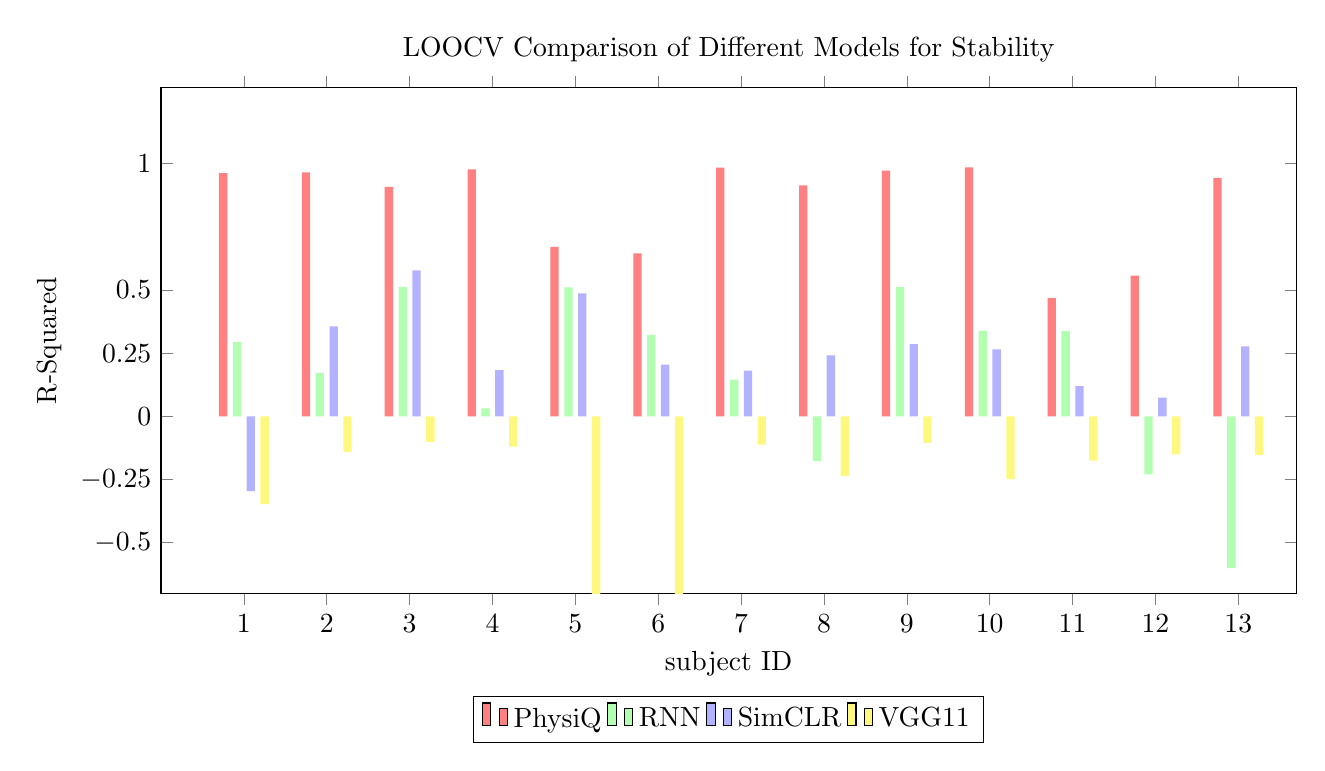
\begin{tikzpicture}
\begin{axis}[
    ybar,
    title=LOOCV Comparison of Different Models for Stability,
% 	x tick label style={
% 		/pgf/number format/1000 sep=},
	xlabel=subject ID,
	ylabel=R-Squared,
xtick={1,2,3,4,5,6,7,8,9,10,11,12,13},
ytick={-.5,-.25, 0, 0.25,  .5, 1.0},
% axis equal,
bar width=3pt,
height=8cm,width=16cm,
% 	enlargelimits=.1,
xmin=0, xmax=13.7, ymin=-.7, ymax=1.3,
	legend style={at={(0.5,-.25
	)},
	anchor=center,legend columns=-2},
% 	nodes near coords,  
%     nodes near coords align={vertical},  
% 	ybar interval=.4,
]
\addplot[draw=none, fill=red!50]  
%PhysiQ with attention
	coordinates {
	(1, 0.962759)
(2, 0.965883)
(3, 0.908476)
(4, 0.977755)
(5, 0.670809)
(6, 0.645153)
(7, 0.984199)
(8, 0.913709)
(9, 0.972433)
(10, 0.985297)
(11, 0.46807)
(12, 0.557421)
(13, 0.943878)
% python .\siamese_cross_validation.py --exercise sa --metrics stability  --lr .001 --hidden_size 256 --epochs 25 --dropout .2
% \begin{comment}
% average 0.8427571601500191
% (3, 0.962759, 0.00230378)
% (8, 0.965883, 0.0021105)
% (9, 0.908476, 0.00566173)
% (10, 0.977755, 0.00137607)
% (11, 0.670809, 0.020364)
% (12, 0.645153, 0.0219511)
% (13, 0.984199, 0.000977434)
% (14, 0.913709, 0.00533803)
% (15, 0.972433, 0.00170533)
% (16, 0.985297, 0.000909541)
% (17, 0.46807, 0.0329056)
% (18, 0.557421, 0.0273783)
% (19, 0.943878, 0.00347175)
% \end{comment}

};
\addplot[draw=none, fill=green!30]
	coordinates {
(1, 0.294923) 
(2, 0.17256) 
(3, 0.512831) 
(4, 0.0316302) 
(5, 0.510665) 
(6, 0.322193) 
(7, 0.145134) 
(8, -0.177127) 
(9, 0.511648) 
(10, 0.337905) 
(11, 0.337649) 
(12, -0.22917) 
(13, -0.600711) 
};

% average 0.16693313646634234
% (3, 0.294923, 0.0105827) 
% (8, 0.17256, 0.0124193) 
% (9, 0.512831, 0.00731207) 
% (10, 0.0316302, 0.0145346) 
% (11, 0.510665, 0.00734459) 
% (12, 0.322193, 0.0101734) 
% (13, 0.145134, 0.012831) 
% (14, -0.177127, 0.0176679) 
% (15, 0.511648, 0.00732984) 
% (16, 0.337905, 0.0099376) 
% (17, 0.337649, 0.00994145) 
% (18, -0.22917, 0.018449) 
% (19, -0.600711, 0.0240256) 
\addplot[draw=none, fill=blue!30]
	coordinates {
(1, -0.295405) 
(2, 0.356205) 
(3, 0.577606) 
(4, 0.183517) 
(5, 0.486332) 
(6, 0.204654) 
(7, 0.180871) 
(8, 0.241452) 
(9, 0.286067) 
(10, 0.265597) 
(11, 0.119688) 
(12, 0.0739067) 
(13, 0.276641) 
 };
\addplot[draw=none, fill=yellow!50] 
	coordinates {
(1, -0.347592) 
(2, -0.140759) 
(3, -0.101083) 
(4, -0.119998) 
(5, -0.735928) 
(6, -0.872492) 
(7, -0.111727) 
(8, -0.236336) 
(9, -0.104602) 
(10, -0.248734) 
(11, -0.174895) 
(12, -0.150518) 
(13, -0.152214) 
 };
	
\legend{PhysiQ, RNN, SimCLR, VGG11}

\end{axis}
\end{tikzpicture}
\caption{We also show the performance of shoulder abduction with the metrics of \textit{stability}. PhysiQ, shown in red, has perform significantly better than other models.}
\label{fig:stability}
\end{figure}